% Created 2019-05-02 Thu 12:56
% Intended LaTeX compiler: pdflatex
\documentclass[11pt]{article}
\usepackage[latin1]{inputenc}
\usepackage[T1]{fontenc}
\usepackage{graphicx}
\usepackage{grffile}
\usepackage{longtable}
\usepackage{wrapfig}
\usepackage{rotating}
\usepackage[normalem]{ulem}
\usepackage{amsmath}
\usepackage{textcomp}
\usepackage{amssymb}
\usepackage{capt-of}
\usepackage{hyperref}
\author{Yelugoti Mohana Datta - IMT2016012}
\date{\today}
\title{On the Design of Display Processors}
\hypersetup{
 pdfauthor={Yelugoti Mohana Datta - IMT2016012},
 pdftitle={On the Design of Display Processors},
 pdfkeywords={},
 pdfsubject={},
 pdfcreator={Emacs 26.2 (Org mode 9.1.9)}, 
 pdflang={English}}
\begin{document}

\maketitle

\section{Authors}
\label{sec:orgc19242e}

This paper was written by T.H Myer and I.E Sutherland with inputs from
Bolt Beranek and Newman Inc.

\begin{itemize}
\item I.E Sutherland is a computer scientist and Internet pioneer, he was 
widely regarded as \uline{father of computer graphics}.

\item He received Turing award from Association for Computing Machinery in
\uline{1988} for invention of sketchpad, an early predecessor to GUI.
\end{itemize}

\subsection{Sketchpad}
\label{sec:org2b2c962}
\begin{center}
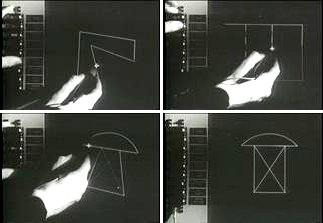
\includegraphics[width=.9\linewidth]{./images/spad.jpg}
\end{center}
\section{Introduction}
\label{sec:org38e7b54}

This paper talks about the flexibility and power needed in the data
channel for computer display, it also looks at the design of the 
display processor (control part of the display) and how it was 
found that making successive improvements to design of display processor
lie on a circular path. It also talks about the various challenges faced
in associating the display with the core computer.

\subsection{Context}
\label{sec:org040d647}

\begin{itemize}
\item The display that the authors are designing is for SDS-940 time shared 
computer system.

\begin{itemize}
\item SDS-940 was the first machine designed to directly support
time-sharing. (Multiple users using single machine)
\end{itemize}
\end{itemize}


\subsection{TX-O display}
\label{sec:org146292d}

\begin{figure}[htbp]
\centering
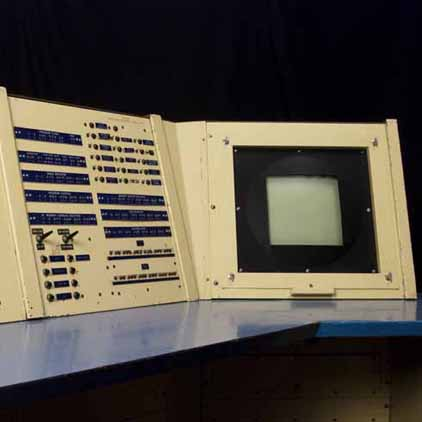
\includegraphics[width=.9\linewidth]{./images/TX-0.jpg}
\caption{TX-0 display}
\end{figure}

\subsection{DEC-PDP}
\label{sec:orge68286a}
\begin{figure}[htbp]
\centering
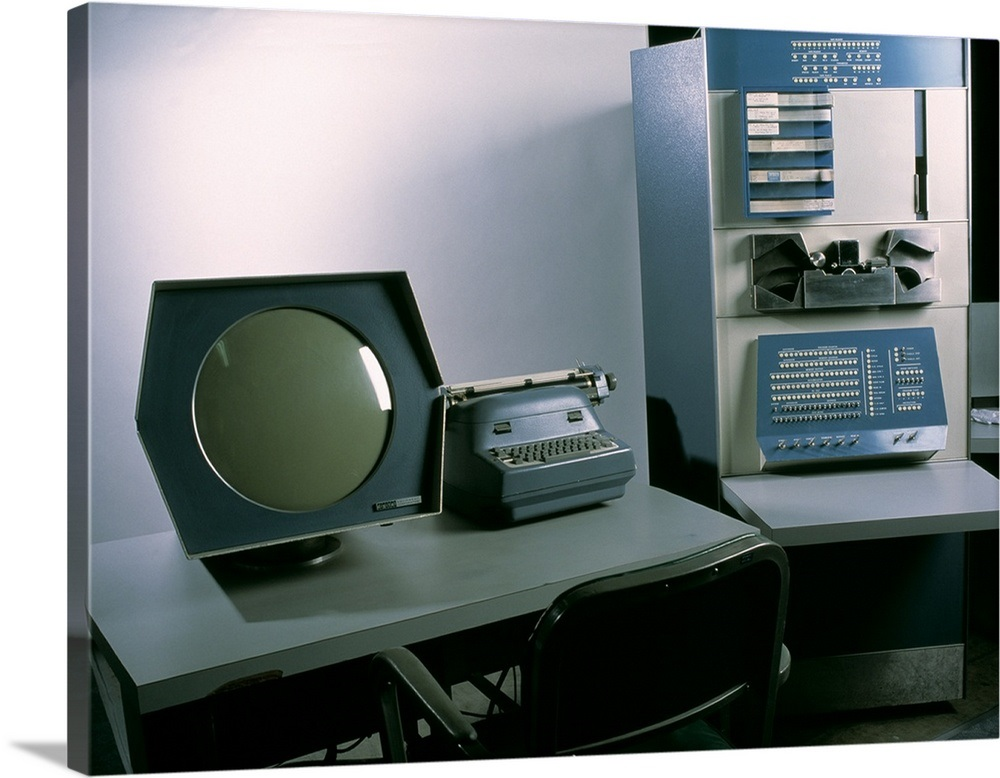
\includegraphics[width=.9\linewidth]{./images/pdp-1.jpg}
\caption{DEC-PDP}
\end{figure}
\section{The Wheel of Reincarnation}
\label{sec:org6a67b8e}

When the authors decided to design the display processor, it got so complex
and it resembled a full fledged computer with some special graphic features,
and then a strange thing happened, the authors were compelled to add a 
second, subsidary processor, which itself began to grow in size, it continued
and authors found that they were stuck in this never ending cyclic process.
They called it wheel of Reincarnation.

\subsection{Stages:}
\label{sec:org1d63e42}

\begin{itemize}
\item Display from core's central registers.
\item Introducing a data channel.
\item Drawing lines and characters.
\item Introducing
\begin{itemize}
\item HALT command.
\item JUMP command.
\item Subroutine feature for repetitive symbols.
\item Store-exit command.
\end{itemize}
\end{itemize}

\subsection{Realisation:}
\label{sec:orga5306df}

We should realize that display data channel is not a mere data channel,
but is a processor.

\begin{center}
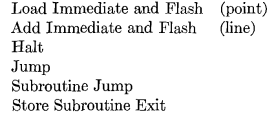
\includegraphics[width=.9\linewidth]{./images/reali.png}
\end{center}

\subsection{Further improvements:}
\label{sec:org09d79de}

\begin{itemize}
\item Introducing stack.
\item Adding conditional commands for interactive programs.
\item Transparency by parameter passing.
\item Global variables support.
\end{itemize}

\subsection{Full-Blown processor}
\label{sec:orgacdf4b7}

\begin{center}
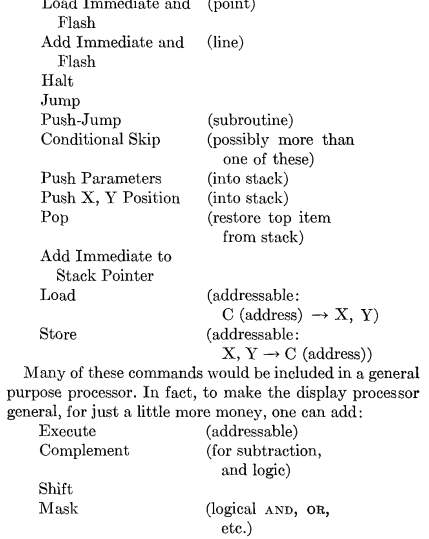
\includegraphics[width=.9\linewidth]{./images/rel2.png}
\end{center}

\subsection{}
\label{sec:org71ea435}

So, if we take a look at the design, we have built up display channel
until it itself is a general purpose processor with a display. The
display is tied directly to its processor, to generate a picture the
display processor's central registers are used. In short, we have come
\uline{exactly around once} the wheel of reincarnation.

However, we have made significant developement, we have added support
for many things in the process.

\subsection{}
\label{sec:orgd488c35}

Now, we might argue that much of display processor's power is idle most
of the time and that it is wasteful to tie up a general purpose processor
merely to refresh a static display, therefore we might consider adding
a \emph{channel} to display processor, which can have some special commands
to let it follow more complex data structures, \textbf{but} if we do this, we 
would be move into a second turn around the wheel.

Looking at commercial displays at that time, one can find many examples
at various points around the wheel, but none stopping exactly at one
revolution around the wheel.
\section{General Questions}
\label{sec:orgbd9c25c}

\subsection{Questions:}
\label{sec:org2bcb44f}

Viewing this from a broader view, we see that there are mainly two
questions:

\begin{itemize}
\item How closer should the display system be tied to parent systems?
\item How much computing power should be included in the display processor?
\end{itemize}

The authors favor keeping the display close to the parent system,
inspite of memory problems (if it had been far, it would have separate
memory and we wouldn't face these).

\subsection{How much computing power?}
\label{sec:org38a81ab}

Depends on what we want to do with our display processor.

\begin{itemize}
\item The display processor must generate pictures from some form of 
internal representation, which may include multiple calls
on display subroutines.
\item Display element might generate pictures from computation rather
than static representation in memory. (light-pens etc)
\item Display processor might provide immediate feedback to user or handle
simple interactive functions such as editing, light-pen tracking.
\item The display processor should handle rotation, scaling etc when
these are not handled by the display hardware.
\end{itemize}
\subsection{Escaping the wheel}
\label{sec:org7de1e09}

The view suggested by Daniel Bobrow that the display processor need
not contain general purpose computing power, largely determined the
design of the display processor.

General computing power should come from central resources of the
system, if there are no enough resources to do particular thing it's
fault of the system not the display. The display should mostly be concerned
with displaying the points. This decision let's us escape from
the wheel of reincarnation.
\section{References:}
\label{sec:orgd41ba6c}

\begin{itemize}
\item \url{https://www.greatbigcanvas.com/view/dec-pdp-1-computer,1154199/}
\item \url{https://en.wikipedia.org/wiki/History\_of\_computing\_hardware}
\item \url{https://archive.org/stream/sds-940/Image071017220051\_djvu.txt}
\item \url{https://en.wikipedia.org/wiki/Display\_Data\_Channel}

\textbf{\uline{Thank you!}}
\end{itemize}
\end{document}
